\FILE{quickstart.tex}

\section{Cloudmesh-cc Interfaces}

In this section we explain the various ways of interfacing with cloudmesh-cc.

It is important to note that we have a {\em commandline mode} that interfaces directly with the backends while not requiering a service. This includes an easy to use python API.

In addition we have used this API to implement a {\em service mode}, so we an stand up a REST service as well as a GUI that can ba accessed through a Web browser.
Please note that the service mode can also be access through te command line in a terminal. To distinguish how we operate cloudmesh-cc we use the term {\em mode} to deliniate it from a command that is entered ina terminal to query the status of the workflow.

We will now discuss tes interfaces in more detail and also showcase
hwo we can access them.


\subsection{Python API}

Cloudmesh-cc is implemented in Python. Extensive documentation is
available in GitHub and through GitHub action it is automatically
updated \cite{github-cloudmesh-cc}.  We distingush two main classes
that are easy to use. The first is a {\em Job class} that can adapted
to include new computational resource types for executing jobs. The
second is a {\em Workflow class} to ccordinate the execution of
multiple jobs. Selected methods of the Job class include are listed in
Figure~\ref{fig:code-job}. Importat to note is that the code for the
scripts are all managed locally and a syncronization step is invoked
prior to one running the job as to assuer that the lates script and
code to be executed on the compute resource is available.

\begin{figure}[htb]
\caption{Pseudo code for the Job class with selected methhods}
\label{fig:code-job}
\begin{minted}[breaklines]{bash}
class Job:
   ...
   def clear():
      """clear job progress"""
   def create(filename=None, script=None, exec=None):
      """Create a template for the script with progress."""
   def get_log(refresh=True):
      """Get the log of the job."""
   def get_pid(refresh=False)
      """Get the pid that the job is running within determined  by the compute resource it is running on""".
   def get_progress(refresh=False):
       """Get the progress of the job from the compute resource."""
   def get_status(refresh=False):
       """Get the status of the job."""
   def kill()
       """Kill the job."""
   def run():
       """Run the job."""
   def sync():
       """Synchronise the current directory with the remote. Copies the shell script to the experiment directory and ensures that the file is copied with the sync command
   def watch(period=10)
       """Watch the job and check for changes in the given period."""

\end{minted}
\end{figure}

\begin{figure}[htb]
\caption{Pseudo code for the Job class with selected methhods}
\label{fig:code-workflow}
\begin{minted}[breaklines]{bash}

class Workflow(...):


    Workflow class that runs all jobs, handles dependencies, etc.


    Initialize a workflow with specified characteristics.

    Parameters

            name (str) – name of workflow

            filename (str) – location of yaml file to load workflow from

            runtime_dir (str) – directory of yaml file to be read and written to

            user (str) – name of user

            host (str) – location of where the workflow will be run

            load (bool) – whether to load the workflow

    add_dependencies(dependency)

        Add a job dependency to the workflow (and the graph).

        Parameters

            dependency (str) – the dependency to be added
        Returns

            nothing
        Return type

            None

    add_dependency(source, destination)

        Add a job dependency to the workflow (and the graph).

        Parameters

                source (str) – job to be completed first

                destination (str) – job to be completed after the source

        Returns

            nothing
        Return type

            None

    add_job(filename=None, name=None, user=None, host=None, label=None, label_format=None, kind='local', status='ready', progress=0, script=None, exec=None, pid=None, venv=None, **kwargs)

        Add a job to the workflow.

        Parameters

                name (str) – name of job

                user (str) – username for job

                host (str) – where the job will be run

                label (str) – what the node will say on the graph

                label_format – how the label will be formatted in the graph

                kind (str) – the type of job, such as local, ssh, slurm

                status (str) – how the job is doing, like ready, failed, done

                progress (int) – a number from 0 to 100 that reports job completeness

                script (str) – the script that the job will run

                exec (str) – how the job will be executed

                pid (int or str) – process id of the job

                kwargs (kwargs) – any other miscellaneous specifications for the job

        Returns

            nothing
        Return type

            None

    analyze_states()

        Return a wordcount on status.

        Returns

            dict of occurrences of each status
        Return type

            dict

    create_topological_order()

        Update the graph while each node bget a number determined from get_sequential_order.

        Returns

            list depicting the workflow
        Return type

            list

    property dependencies

        Retrieve the dependencies of the workflow.

        Returns

            the dependencies of the workflow
        Return type

            dotdict

    property dict_of_workflow

        Return a dict of the nodes and dependencies of the workflow.

        Returns

            dict of workflow
        Return type

            dict

    display(filename=None, name='workflow', first=True)

        Show the graph of the workflow.

        Parameters

                filename (str) – location of the graph

                name (str) – name of the workflow to be displayed

                first (bool) – if True then this is first time graph is displayed

        Returns

            nothing
        Return type

            None

    get_predecessors(name)

        Return the predecessors.

        Figure out all the dependencies of the name node then test if each node in front (parent) has progress of 100 if the parent has progress 100, remove those nodes.

        Parameters

            name (str) – name of a job
        Returns

            list of preceding jobs
        Return type

            list

    job(name)

        Return the details of a job within the workflow.

        Parameters

            name (str) – name of job
        Returns

            details of a job within the workflow
        Return type

            dict

    property jobs

        Retrieve the jobs of the workflow.

        Returns

            the jobs that belong to the workflow
        Return type

            dotdict

    json(filepath=None)

        Return the workflow as json string.

        Parameters

            filepath (str) – where the file is located
        Returns

            a json string of the workflow
        Return type

            str

    load(filename, clear=True)

        Load the workflow.

        Load a workflow graph from file. However, the file is still stored in the filename that was used when the Workflow was created. This allows to load in a saved workflow in another file, but continue working on it in the file used in init.

        Parameters

                filename (str) – which file to load the workflow from

                clear (bool) – whether to clear workflow. not implemented

        Returns

            nothing
        Return type

            None

    load_with_state(filename)

        Load the workflow with state.

        Parameters

            filename (str) – which file to load the workflow from
        Returns

            nothing
        Return type

            None

    predecessor(name)

        Retrieve the jobs that must be run before the specified job.

        Parameters

            name (str) – name of a job
        Returns

            list of preceding jobs
        Return type

            list

    remove_job(name, state=False)

        Remove a particular job from the workflow.

        Parameters

                name (str) – name of job to be removed from workflow

                state (bool) – whether to save workflow with state after job removal

        Returns

            nothing
        Return type

            None

    remove_workflow()

        Delete workflow from the local file system.

        Returns

            nothing
        Return type

            None

    run_parallel(directory='~/experiment', order=None, dryrun=False, show=True, period=0.5, filename=None)

        Run a workflow in a parallel fashion.

        Parameters

                directory (str) – where the workflow should be run

                order – how the jobs should be run chronologically

                dryrun (bool) – if true then the workflow isn’t really run. for testing

                show (bool) – whether to show graph as workflow is run

                period (float) – how long to wait after showing the graph

                filename (str) – where to save the graph

        Returns

            nothing
        Return type

            None

    run_topo(order=None, dryrun=False, show=True, filename=None)

        Run the workflow in a topological fashion.

        Parameters

                order – how the jobs should be run chronologically

                dryrun (bool) – if true then the workflow isn’t really run. for testing

                show (bool) – whether to show the graph as workflow is run

                filename (str) – where the graph should be saved

        Returns

            nothing
        Return type

            None

    save(filename=None)

        Save the workflow.

        Parameters

            filename (str) – where to save the workflow
        Returns

            nothing
        Return type

            None

    save_with_state(filename, stdout=False)

        Save the workflow with state.

        Parameters

                filename (str) – which file to save the workflow

                stdout (bool) – if True then return the output

        Returns

            if stdout is True then returns the string of yaml dump
        Return type

            None or str

    sequential_order()

        Return a list of the topological order of the workflow.

        Returns

            list depicting the workflow
        Return type

            list

    set_progress(name, percent)

        Manually update a job’s progress.

        Parameters

                name (str) – name of the job

                percent (int) – value from 0 to 100 for the progress

        Returns

            nothing
        Return type

            None

    status()

        Return details of the workflow in dict format.

        Returns

            details of workflow in dict format
        Return type

            dict

    property table

        Return a table of the workflow.

        Returns

            a table of the workflow
        Return type

            None or PrettyTable or str or dict

    table2(with_label=False)

        Return a table of the workflow.

        Parameters

            with_label (bool) – whether to include label in table
        Returns

            a table of the workflow
        Return type

            None or PrettyTable or str or dict

    update_progress(name)

        Manually update the progress of a job according to its log file.

        Parameters

            name (str) – name of job
        Returns

            nothing
        Return type

            None

    update_status(name, status)

        Manually update a job’s status.

        Parameters

                name (str) – the job whose status will be updated

                status (str) – the new status to be set for the job

        Returns

            nothing
        Return type

            None

    property yaml

        Return a yaml dump of the nodes and dependencies of the workflow.

        Returns

            yaml dump of workflow as string
        Return type

            str

cloudmesh.cc.workflowrest module

Cloudmesh cc REST workflow.



\end{minted}



\begin{figure}[htb]
\caption{Pseudo code for the Job class with selected methhods}
\label{fig:code-workflow-rest}
\begin{minted}[breaklines]{bash}

class RESTWorkflow

    Bases: object

    Class which interfaces with cc FastAPI server using REST.

    Initialize the service.

    add_job(workflow_name, **kwargs)

        Add a job to the workflow.

        Adds a job to a workflow that is specified in the provided workflow_name string.

        Returns

            all jobs within workflow
        Return type

            dict

    delete_workflow(workflow_name, job_name=None)

        Delete a workflow by using REST.

        Parameters

                workflow_name (str) – name of workflow to delete

                job_name (str) – name of job to delete inside specified workflow

        Returns

            success or failure message
        Return type

            dict

    def get_workflow(workflow_name, job_name=None):
        Retrieve a workflow by using REST.

    def list_workflows():
        """Return a list of workflows that is found within the server."""

    def run_workflow(workflow_name, run_type='topo', show=True):
        """Run a workflow by using REST."""

    def upload_workflow(directory=None, archive=None, yaml=None):
        """Upload a workflow by using REST."""
\end{minted}

\begin{figure}[htb]
\caption{Pseudo code for the Job class with selected methhods}
\label{fig:code-workflow-example}
\begin{minted}[breaklines]{bash}
    w = Workflow(filename="workflow.yaml")
    w.load(filename="abc.yaml") <- loads in the graph, but will save it still to workflow.yaml
    w.add(filename="add.yaml") <-adds a new workflow into the existing one.
    w.add_job(name="a",
                command="hostname",
                user=None, # bug if kind is local and user is None, we do not need user, but can take local user
                host=None, # bug:  if host is none and kind is local use localhost
                label="a",
                kind="local",
                status="ready",
                progress=0)
    w.add_job(name="b", command="ls")
    w.add_job(name="c", command="pwd")
    w.add_job(name="d", command="uname -a")
    w.add_dependencies(dependency="a,b,d")
    w.add_dependencies(dependency="a,c,d")

    w.run()
\end{minted}


\subsection{Commandline Mode}

The commandline mode is a an implementation that does not use a
backend service. It runs in the terminal till the workflow is
completed. All state of the jobs are managed on the compute service on
which the job is run and the status is replicated into the client on
demand. THis allows easy reporting of the statsu through a table and a
graph display using client based rendering tools. 


The Cloudmesh Compute Cluster service allows you to execute analytical,
computational workflows which run programs on remote compute resources.
We specify not only a list of tasks to be executed, but the tasks can
also have dependencies between each other expressed through a direct,
cyclic graph. Currently, we have predefined task types that can execute
shell scripts, Python programs, and Python notebooks, all of which can
be executed on local or remote compute resources.


We can specify such workflows in a YAML file making it very easy to
create and manage them. To get you started, we have developed a
quickstart example that you can enhance to get acquainted with the
system.

Once a workflow is specified, it can be executed a using one of our
interfaces. This includes a Python API and a command line interface
without a REST service. In addition we have, with the help of the Python
API, developed a REST service so that integration into other frameworks
can be facilitated through REST calls. The availability of the REST
service is important to access it from non Python frameworks, but also
allows the easy interaction through a Web-based Portal.

Let us demonstrate a number of selected features with the help of this
quickstart. We will only focus on using the REST service.

\subsection{Setup}\label{setup}

To start, the code is needed and we assume you are standing in the
cloudmesh-cc directory. Use the following commands

\smallskip
\begin{minted}[breaklines]{bash}
$ git clone https://github.com/cloudmesh/cloudmesh-cc.git
$ cd cloudmesh-cc
$ pip install -e .
\end{minted}
\smallskip

We also assume you start the service with

\smallskip
\begin{minted}[breaklines]{bash}
$ cms cc start --reload
\end{minted}
\smallskip

\subsection{Creating a simple example}\label{creating-a-simple-example}

First let us create a simple workflow example that we already have
included for you in our source code. We will use this workflow and copy
it into a temporary directory:

\smallskip
\begin{minted}[breaklines]{bash}
$ mkdir -p /tmp/workflow-example
$ cp tests/workflow-example/workflow-example.yaml /tmp\
/workflow-example
$ cp tests/workflow-example/*.sh /tmp/workflow-example
\end{minted}
\smallskip

\TODO{create refs, only one for the dir and than we can refer to the others as is, we nit github ref}

We like you to inspect the example so you get an overview of how to
define a workflow that is located in
\href{https://github.com/cloudmesh/cloudmesh-cc/tree/main/tests/workflow-example}{GitHub} and is located in the folder \emph{tests/workflow-example/}

\begin{itemize}
\item
  \href{https://github.com/cloudmesh/cloudmesh-cc/blob/main/tests/workflow-example/workflow-example.yaml}{workflow-example.yaml}
\item
  \href{https://github.com/cloudmesh/cloudmesh-cc/blob/main/tests/workflow-example/fetch-data.sh}{fetch-data.sh}
\item
  \href{https://github.com/cloudmesh/cloudmesh-cc/blob/main/tests/workflow-example/compute.sh}{compute.sh}
\item
  \href{https://github.com/cloudmesh/cloudmesh-cc/blob/main/tests/workflow-example/analyze.sh}{analyze.sh}
\end{itemize}

Now we can test a selected number of ways on how to interact with the
service. We showcase here how to

\begin{itemize}
\item
  \begin{enumerate}
  \def\labelenumi{\Alph{enumi}.}
  \item
    upload workflows as tar/xz file of a self containing directory, or
  \end{enumerate}
\item
  \begin{enumerate}
  \def\labelenumi{\Alph{enumi}.}
  \setcounter{enumi}{1}
  \item
    upload all files in a directory recursively
  \end{enumerate}
\end{itemize}

\subsection{A. Upload and run a workflow embedded in an archive
file}\label{a.-upload-and-run-a-workflow-embedded-in-an-archive-file}

We can upload an archive file which contains all the workflow files,
including the yaml specification file and the scripts. Providing an
archive file such as a \mintinline{bash}|.tar|, \mintinline{bash}|.tar.gz|, or \mintinline{bash}|.xz|.
may enable the workflow to be better suited towards portability and
simplicity, where one can share an archive file with another user. We
will choose here a tar file as example.

\subsubsection{Create tar archive file}\label{create-tar-archive-file}

Before uploading a \texttt{tar} archive file, we must first create it
using the previous example yaml and scripts that we copied.

\smallskip
\begin{minted}[breaklines]{bash}
$ tar -C /tmp/workflow-example -cf workflow-example.tar .
\end{minted}
\smallskip

\subsubsection{\texorpdfstring{Option 1: Upload via
\texttt{curl}}{Option 1: Upload via curl}}\label{option-1-upload-via-curl}

We can upload the archive file by using the \texttt{curl} terminal
command as follows:

\smallskip
\begin{minted}[breaklines]{bash}
$ curl -X 'POST' 'http://127.0.0.1:8000/ workflow?archive=workflow-example.tar'     -H 'accept: application/json' -d ''
\end{minted}
\smallskip

\subsubsection{\texorpdfstring{Option 2: Upload via
\texttt{/docs}}{Option 2: Upload via /docs}}\label{option-2-upload-via-docs}

As the service is using also an OpenAPI 2.0 specification the workflow
can also be uploaded implicitly through the specification GUI. Navigate
to \texttt{http://127.0.0.1:8000/docs} and use the POST Upload method.

\begin{figure}
\centering
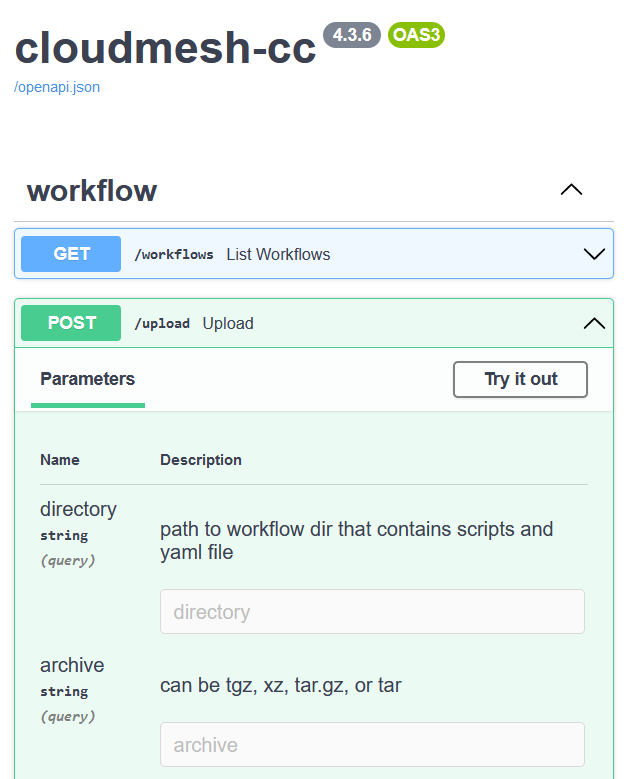
\includegraphics[width=0.7\columnwidth]{images/upload_api.png}
\caption{Browser API GUI for Cloudmesh Compute Cluster}
\end{figure}

Please click \texttt{Try\ it\ out} and then enter \newline
\mintinline{bash}|~/cm/cloudmesh-cc/workflow-example.tar| in the
\mintinline{bash}|archive| field and then click Execute.

\subsubsection{Option 3: Upload via the Python
API}\label{option-3-upload-via-the-python-api}

As we use a REST service, we can also easily upload the workflow through
a Python enabled REST call. We will use Python requests to demonstrate
this upload feature.

\smallskip
\begin{minted}[breaklines]{python}
import requests

r = requests.post('http://127.0.0.1:8000/ workflow?archive=workflow-example.tar')
print(r)
print(r.text)
\end{minted}
\smallskip

Printing \texttt{r} returns the response code from the API (a code of
200 indicates success). Printing \texttt{r.text} returns the message
from the API, such as a success or error message.

\subsubsection{Option 4: Upload with a third party REST
framework}\label{option-4-upload-with-a-third-party-rest-framework}

Naturally if you like to use a different REST API you can do so. You can
also use different programming languages and we leave it up to you to
choose the framework of your choice to interact with the REST service,
popular choices are JavaScript, Go, C/C++, matlab, and R, to name a few.

\subsection{B. Upload a dir that contains workflow
directory}\label{b.-upload-a-dir-that-contains-workflow-directory}

To increase flexibility and allow quick experiments, users can specify a
workflow directory which contains the yaml specification file and the
scripts. This way, pre-archival of the directory is not needed. The
program sets up the workflow by copying the necessary files from the
specified directory.

There are three different ways to upload the dir: via \texttt{curl} on
the command line, via the browser GUI, and via the Python API.

\subsubsection{\texorpdfstring{Option 1: Upload via
\texttt{curl}}{Option 1: Upload via curl}}\label{option-1-upload-via-curl-1}

A workflow can be uploaded easily with a curl command from the command
line. On the command line execute:

\smallskip
\begin{minted}[breaklines]{bash}
$ curl -X 'POST' 
  'http://127.0.0.1:8000/workflow?directory= ~/cm/cloudmesh-cc/tests/workflow-example' 
  -H 'accept: application/json' 
  -d ''
\end{minted}
\smallskip

\subsubsection{\texorpdfstring{Option 2: Upload via
\texttt{/docs}}{Option 2: Upload via /docs}}\label{option-2-upload-via-docs-1}

Also here one can upload the needed files with the OpenAPI specification
interface on the service. Navigate to
\mintinline{bash}|http://127.0.0.1:8000/docs| and use the POST Upload method. 
Click \mintinline{bash}|Try it out| and then enter

\begin{minted}[breaklines]{bash}
/cm/cloudmesh-cc/tests/workflow-example
\end{minted}

in the
directory field and then click Execute.

\subsubsection{Option 3: Upload via the Python
API}\label{option-3-upload-via-the-python-api-1}

Accessing the upload from the Python API is very easy. We will use
python requests to demonstrate the upload of the workflow.

\smallskip
\begin{minted}[breaklines]{python}
import requests
r = requests.post('http://127.0.0.1:8000 /workflow?directory= ~/cm/cloudmesh-cc/tests/workflow-example')
print(r)
print(r.text)
\end{minted}
\smallskip

Printing \mintinline{bash}|r| returns the response code from the API (a code of
200 indicates success). Printing \mintinline{bash}|r.text| returns the message
from the API, such as a success or error message.

\subsection{Parameters to the Upload a workflow with a REST
call}\label{parameters-to-the-upload-a-workflow-with-a-rest-call}

The upload REST URL can take different parameters, such as

\begin{minted}[breaklines]{bash}
directory=name
archive=name.tar.gz
archive=name.tgz
archive=name.xz
yaml=name
\end{minted}

The semantic of the upload is specified through its parameter. Only one
of them can be used at a time.

The directory parameter indicates that the contents of a specified
directory will be transferred into a workflow.

The archive parameter indicates that an archive file, such as a
\texttt{tar} file, will be extracted and its contents will be
transferred into a workflow. Please note that the \texttt{archive} and
\texttt{directory} parameters can not be used in the same REST call.

The yaml parameter indicates that only a yaml file will be uploaded
without any corresponding scripts. Uploading a yaml file by itself
allows for a script specified by the yaml to be uploaded later. The yaml
can even work without scripts by using the \texttt{exec} specification
within the yaml.

\subsection{Run the workflow}\label{run-the-workflow}

To run, navigate to homepage at \texttt{http://127.0.0.1:8000/} and
click the workflow-example on the left side. Then click Run.
